\documentclass[runningheads]{llncs}
\usepackage{graphicx}
\usepackage{cite}
\usepackage[verbose]{wrapfig}
%\usepackage{hyperref}

\begin{document}

\title{Object-Oriented Internet\\ Cloud Interoperability}
%\titlerunning{OOI - Cloud Interoperability}

\author{Mariusz Postół\inst{1}\orcidID{0000-0002-9669-0565}  \and Piotr Szymczak\inst{1}\orcidID{0000-0001-6790-3878} }
%\authorrunning{M. Postół et al.}

\institute
{ Institute of Information Technology, Lodz University of Technology, Łódź, Poland \\
      \email{mailto:mariusz.postol@p.lodz.pl} %\\ \url{http://www.it.p.lodz.pl}
}

\maketitle

\begin{abstract}

      Optimization of the industrial processes requires further research on the integration of machine-centric systems with human-centric cloud-based services in the context of new emerging disciplines, namely Industry 4.0 and Industrial Internet of Things. This research aims at working out a new generic architecture and deployment scenario applicable to this integration. The reactive interoperability relationship of the interconnected nodes is proposed to deal with the network traffic propagation asymmetry or assets' mobility. Described solution based on the OPC Unified Architecture international standard relaxes issues related to the real-time multi-vendor environment. The discussion addressing the generic architecture concludes that the embedded gateway software part best suits all requirements. To promote separation of concerns and reusability, the proposed architecture of the embedded gateway has been implemented as a composable part of a selected OPC UA PubSub framework.

      The proposals are backed by proof of concept reference implementations confirming the possibility to integrate selected cloud services with the cyber-physical system interconnected as one whole atop of the OPC UA by applying the proposed architecture and deployment scenario. It is contrary to interconnecting cloud services with a selected OPC UA server limiting the PubSub role to data export only.

      \keywords{Industry 4.0 \and Internet of Things \and Object-Oriented Internet \and Cloud Computing \and Industrial communication \and Reactive networking \and Machine to Machine Communication \and OPC Unified Architecture \and Azure}

\end{abstract}

\section{Introduction}\label{introduction}

All the time, the Information and Communication Technology is providing society with a vast variety of new distributed applications aimed at micro and macro optimization of the industrial processes. Obviously, the design foundation of this kind of application has to focus primarily on communication technologies. Based on the role humans take while using these applications they can be grouped as follows:

\begin{itemize}
      \item \textbf{human-centric} - information origin or ultimate information destination is an operator,
      \item \textbf{machine-centric} - information creation, consumption, networking, and processing are achieved entirely without human interaction.
\end{itemize}

A typical \textbf{human-centric} approach is a web-service supporting, for example, a web user interface (UI) to monitor conditions and manage millions of devices and their data in a typical cloud-based IoT approach \cite{RefWorks:doc:5d87d02be4b0e88bdacab9a7, RefWorks:doc:5d87d1c9e4b0bc72a68d7b46, RefWorks:doc:5d9216c9e4b03ba5e075a855, 10.1007/978-3-030-50426-7_22}. In this case, it is characteristic that any uncertainty and necessity to make a decision can be relaxed by human interaction. Coordination of robots behavior in a work-cell (automation islands) is a \textbf{machine-centric} example. In this case, any human interaction must be recognized as impractical or even impossible. This interconnection scenario requires the machine to machine communication (M2M) \cite{RefWorks:doc:5d6cdbbbe4b082ad50f3a83e, mpostol2020, RefWorks:doc:5d8f6d9ee4b058d660094a94, RefWorks:doc:5d868e46e4b030b4e0569e60, RefWorks:doc:5d8f7275e4b0bc72a68f4dcb} demanding multi-vendor devices integration.

From the M2M communication concept, a broader idea of a smart factory can be derived. In this M2M  deployment approach, the mentioned robots are only executive assets of an integrated supervisory control system responsible for macro optimization of an industrial process composed as one whole. Deployment of the smart factory concept requires a hybrid solution and interconnection of the mentioned above heterogeneous environments. This approach is called the fourth industrial revolution and was coined as Industry 4.0. It is worth stressing that machines - or more general assets - interconnection is not enough, and additionally, assets interoperability has to be expected for the deployment of this concept. In this case, multi-vendor integration makes communication standardization especially important, namely, it is required that the payload of the message is standardized to be factored on the data-gathering site and consumed on the ultimate destination site.

Highly-distributed solutions used to control real-time process aggregating islands of automation (e.g.~virtual power plants producing renewable energy) additionally must leverage public communication infrastructure, namely the Internet. Internet is a demanding environment for highly distributed process control applications designed atop the M2M communication paradigm because it is globally shareable and can be also used by malicious users. Furthermore, it offers only non-deterministic communication making integration of islands of automation designed against the real-time requirements a demanding task.

Today both obstacles can be overcome, and as examples, we have bank account remote control and voice over IP in daily use. The first application must be fine-tuned in the context of data security, and the second is very sensitive concerning time constraints. Similar approaches could be applied to adopt the well known in process control industry concepts, namely Human Machine Interface (HMI), Supervisory Control and Data Acquisition (SCADA), and Distributed Control Systems (DCS). It is worth stressing that, by design, all of them are designed based on interactive communication. Interactive communication is based on a data polling foundation. In this case, the application must follow the interactive behavioral model, because it actively polls the data source for more information by pulling data from a sequence that represents the process state in time. The application is active in the data retrieval process - it controls the pace of the retrieval by sending the requests at its convenience. After dynamically attaching a new island of automation the control application (responsible for the data pulling) must be reconfigured for this interoperability scenario. In other words, in this case, the interactive communication relationship cannot be directly applied because the control application must be informed on how to pull data from a new source. As a result, a plug and produce scenario \cite{PlugProduceByModellingSkills} cannot be seamlessly applied. A similar drawback must be overcome if for security reasons suitable protection methods have been applied to make network traffic propagation asymmetric. It is accomplished using intermediary devices, for example, firewalls, to enforce traffic selective availability based on predetermined security rules against unauthorized access.

Going further, we shall assume that islands of automation are mobile, e.g.~autonomous cars passing a supervisory controlled service area. In this case, the behavior of the interconnected assets is particularly important concerning the environment in which they must interact. This way we have entered the Internet of Things domain of Internet-based applications.

If we must bother with the network traffic propagation asymmetry or mobility of the asset network attachment-points the reactive relationship could relax the problems encountered while the interactive approach is applied \cite{mpostol2020}. In this case, the sessionless publisher-subscriber communication relationship is a typical pattern to implement the abstract reactive interoperability paradigm. The sessionless relationship is a message distribution scenario where senders of messages, called publishers, do not send them directly to specific receivers, called subscribers, but instead, categorize the published messages into topics without knowledge about which subscribers if any, there may be. Similarly, subscribers express interest in one or more topics and only receive messages that are of interest, without knowledge about which publishers, if any, there are. In this scenario, the publishers and subscribers are loosely coupled i.e they are decoupled in time, space and synchronization \cite{RefWorks:doc:5c44e246e4b0591b15ea9e59}.

If the \textbf{machine-centric} interoperability - making up islands of automation - must be monitored and/or controlled by a supervisory system, the cloud computing concept may be recognized as a beneficial solution to replace or expand the mentioned above applications, i.e.~HMI, SCADA, DCS, etc. Cloud computing is a method to provide a requested functionality as a set of services. There are many examples that cloud computing is useful to reduce costs and increase robustness. It is also valuable in case the process data must be exposed to many stakeholders. Following this idea and offering control systems as a service, there is required a mechanism created on the service concept and supporting abstraction and virtualization - two main pillars of the cloud computing paradigm. In the cloud computing concept, virtualization is recognized as the possibility to share the services by many users, and abstraction hides implementation details.

%Deployment of the hybrid solution providing interoperability of the \textbf{machine - centric} Cyber-Physical System (CPS) \cite{RefWorks:doc:5c458659e4b014f3944f6969} and \textbf{human - centric} cloud-based front-end can be implemented applying the following scenarios: \textbf{direct} or \textbf{gateway} based interconnection (Sect. \ref{cloud-to-sensors-field-level-connectivity}). By design, the \textbf{direct} approach requires that the cloud has to be compliant with the interoperability standard the CPS is built upon - it becomes a consistent part of the CPS. Data models, roles, and responsibility differences of both solutions make this approach impractical or even imposable to be applied in a general case. A more detailed description is covered by the Sect.~\ref{cloud-to-sensors-field-level-connectivity}.

This article addresses further research on the integration of the multi-vendor \textbf{machine-centric} CPS designed atop of M2M communication and emerging cloud computing as a \textbf{human-centric} front-end in the context of the Industry 4.0 (I4.0) and Industrial Internet of Things (IIoT) disciplines. For this integration, a new architecture is proposed to support the reactive relationship of communicating parties. To support the multi-vendor environment OPC Unified Architecture \cite{RefWorks:doc:5ac86c99e4b009947bbb87c6, LiteratureSurveyOnOpenPlatformCommunications, RefWorks:doc:5ac86c99e4b009947bbb87d2} interoperability standard has been selected. Prototyping addresses Microsoft Azure Cloud \cite{MicrosoftAzureIoTPlatform} as an example. The proposals are backed by proof of concept reference implementations - the outcome has been just published on GitHub as the open-source (MIT licensed) \cite{mariusz_postol_2020_4361640}. The proposed solutions have been harmonized with the more general concept called the Object-Oriented Internet (OOI) \cite{mariusz_postol_2020_4361640, RefWorks:doc:5c6912c9e4b0a562a3fc7f5b, RefWorks:doc:5c66740ae4b081adf5804596}.

The main goal of this article is to provide proof that

\begin{itemize}
      \item reactive M2M interoperability based on the OPC UA standard can be implemented as a powerful standalone library without dependency on the Client/Server session-oriented archetype
      \item Azure interoperability can be implemented as an external part employing out-of-band communication without dependency on the OPC UA implementation
      \item the proposed generic architecture allows that the gateway functionality is implemented as composable part at run-time part - no programming required
\end{itemize}

The remainder of this paper is structured as follows. Sect.~\ref{cloud-to-sensors-field-level-connectivity} presents the proposed open and reusable software model. It promotes a reactive interoperability pattern and a generic approach to establishing interoperability-context. A reference implementation of this archetype is described in Sect.~\ref{section.gateway-implementation}. The most important findings and future work are summarized in Sect.~\ref{section.conclusion}.

\section{Sensors to Cloud Interconnection - Architecture}\label{cloud-to-sensors-field-level-connectivity}

%\subsection{Architecture}\label{cloud-to-sensors-field-level-connectivity}

To follow the Industry 4.0 concept a hybrid environment integrating reactive Machine to Machine interconnection and the interactive web-based user interface is required (Sect. \ref{introduction}). The main challenge of the solution in concern is to design a generic but reusable architecture that addresses interoperability of these diverse interconnection scenarios ruled by different requirements, namely:

\begin{itemize}
      \item \textbf{machine-centric} machine to machine real-time mobile interoperability
      \item \textbf{human-centric} cloud-based front-end
\end{itemize}

Interconnection of the reactive \textbf{machine-centric} and interactive \textbf{human-centric} environments can be implemented by applying one of the following scenarios:

\begin{itemize}
      \item \textbf{direct interconnection} (tightly coupled scenario) - cloud-based dedicated communication services are engaged to attach it to the CPS making up a consistent M2M communication network using a common protocol stack
      \item \textbf{gateway based interconnection} (loosely coupled scenario) - native build-in communication services allows attaching the cloud to the CPS using an out-of-bound protocol stack
\end{itemize}

By design, the \textbf{direct interconnection} approach requires that the cloud has to be compliant with the interoperability standard the CPS uses. As a result, it becomes a consistent communication node of the CPS. The decision to follow the \textbf{direct interconnection} scenario must be derived from an analysis of the capabilities of available services in concern. However, for the development strategy of this type of solution, this analysis can be done partially taking into account the following features that can be considered invariable. By design the cloud-based services must be virtual - they are used to handle many solutions at the same time. Furthermore, M2M communication is usually constrained by real-time requirements. The virtualization of cloud services means that they must be very flexible to handle the attachment of new assets proactively (acting in advance) at run time. As a result, the cloud services must be responsible to register and authenticate devices by exposing endpoints in the public network to allow the device to access a provisioning cloud service. It requires that a session over the Internet has to be established by the data holding asset at a preparation step. To meet the requirements of real-time distributed control the CPS may use protocols applicable only to local computer networks (e.g.~multicast IP, Ethernet, TSN \footnote{Time-Sensitive Networking (TSN) Task Group \url{https://1.ieee802.org/tsn/}}, etc.). Because the cloud services support only protocols handling interconnection over the Internet the \textbf{direct interconnection} cannot be applied in a general case.

To support also a local network attachment point, the interaction with the cloud requires remote agents implemented by applying one of the following archetypes:

\begin{itemize}
      \item \textbf{edge device} - remote cloud agent acting as an intermediary for nodes of the CPS
      \item \textbf{field level gateway} - a dedicated custom agent acting as an intermediary for nodes of the CPS
      \item \emph{Embedded Gateway} - a software part composed into a selected node of the \emph{Cyber-physical network} (Fig. \ref{figure1.StrategyDomainModel})
\end{itemize}

\textbf{Edge device} connects directly to the cloud services but acts as an intermediary for other devices called leaf devices. Additionally, it allows the selection of initial data and processing of them using local resources. The \textbf{edge device} may be located close to the leaf devices and attached to the \emph{Cyber-physical network} using protocols applicable only to local computer networks. In this scenario, it is possible to use a custom protocol stack to get connected to the \textbf{edge device} with the cloud and helps to save the bandwidth thanks to sending only the results of local processing. In this approach, the \textbf{edge device} is part of cloud vendor products and cannot be recognized as a generic solution that can be used to connect to other clouds at the same time.

The \textbf{field level gateway} is also build atop of the middleware concept \cite{Sunyaev2020}. The only difference compared with the \textbf{edge device} is a necessity to use officially supported by the cloud vendor services to get connected. In this scenario, the process data simultaneously may be transferred to many clouds provided that the gateway offers this functionality.

\begin{proposition}
      Unlike the above-described solutions, the \emph{Embedded Gateway} is not derived from the middleware concept. A generic domain model for this interconnection is presented in the Fig.~\ref{figure1.StrategyDomainModel}. Promoting separation of concern design principle, the gateway functionality should be implemented as a self-contained software part embedded in the \emph{Networking} service of the \emph{Cyber-physical\ node}. The main functionality of this component is to transfer selected data between \emph{Cyber-physical\ network} using \emph{Networking} services of an existing \emph{Cyber-physical\ node} and \emph{Cloud-based\ front-end} using officially supported by the cloud vendor interconnection services.
\end{proposition}

\begin{wrapfigure}{t}{0.55\textwidth}
      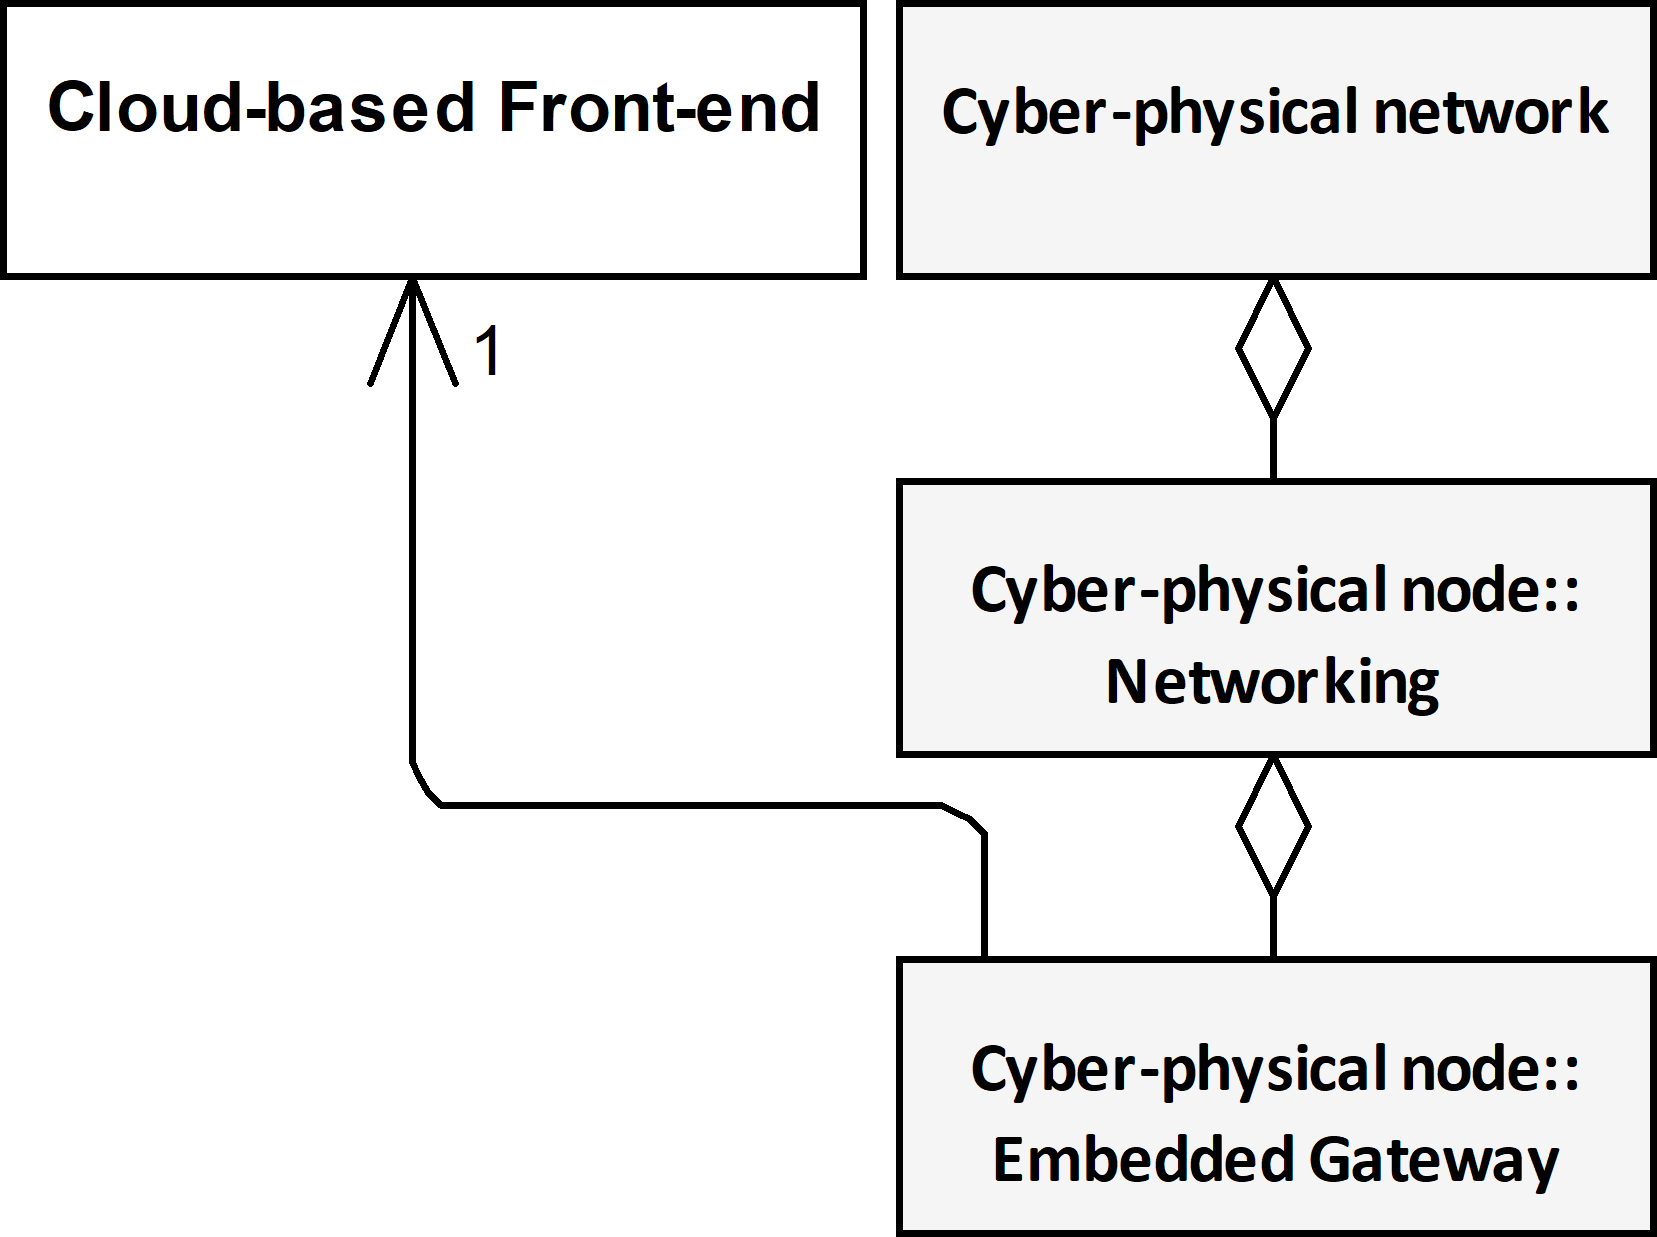
\includegraphics[width=0.53\textwidth]{StrategyDomainModel.eps}
      \caption{Generic interconnection concept}\label{figure1.StrategyDomainModel}
\end{wrapfigure}

% The \emph{Embedded Gateway} archetype relaxes most of the issues described above: \emph{Cyber-physical\ network} real-time behavior, data encoding incompatibility, security - context differences to name only a few. The main goal of this article is to provide proof that the \emph{Embedded Gateway} archetype implementation is possible based on a generic architecture that can be used as a foundation for the integration of the heterogeneous environments in concern. The proposed implementation is designed for a selected interoperability standard and cloud product.

The interconnection of assets is not enough hence their interoperability is expected. In this case, using the same communication stack must be recognized as only a necessary condition. To support interoperability common data understanding is required. Additionally, to meet this requirement the cloud and CPS have to establish directly the same semantic-context and security-context. The possibility to establish a common semantic-context in the multi-vendor environment makes communication standardization especially important. In this case, it is required that the encoding of the payload exchanged over the network (Data Transfer Object) is standardized so that the appropriate messages can be factored on the data-gathering site and consumed on the ultimate destination data processing sites. Security between the data origin and ultimate data destination refers to the protection of messages (security-context) against malicious users. It is required that communicating parties are using the same cyber-security measures. To comply with the Industry 4.0 communication criterion it is required that any product must be addressable over the network via TCP/UDP or IP and has to support the OPC UA Information Model \cite{OPCUAPart5, RefWorks:doc:5ac86c99e4b009947bbb87c9, RefWorks:doc:5d986a28e4b0b0c862c0d184}. As a result, any product being advertised as Industry 4.0 enabled must be OPC UA-capable somehow. 

To support the multi-vendor environment OPC Unified Architecture interoperability standard has been selected. OPC UA supports the following two patterns to be used to transfer data between communicating parties:

\begin{itemize}
      \item \textbf{session-oriented}: requires a session that has to be established before any data can be sent between sender and receiver
      \item \textbf{sessionless-oriented}: the sender may start sending messages (called packets or datagrams) to the destination without any preceding handshake procedure
\end{itemize}

Using the session-oriented communication pattern it is difficult or even impossible to gather and process mobile data (Sec.~\ref{introduction} ), which is one of the Internet of Things paradigms. OPC UA Part 14 PubSub \cite{RefWorks:doc:5d98837de4b055984c0eecf0, UAPart14PubSubMainTechnologyFeatures} offers the sessionless approach as an additional option to session-based client-server interoperability relationship and is a consistent part of the OPC UA specifications suit. As the result, it can be recognized as the IoT ready technology.

The presented proposals in the article are backed by proof of concept reference implementations\cite{mariusz_postol_2020_4361640}. For this study, prototyping addresses Microsoft Azure cloud products. There are many reasons for selecting Azure to accomplish the cloud-based front-end of Cyber-Physical System (CPS). Azure offers Infrastructure as a Service (IaaS) and Platform as a Service (PaaS) capabilities. As a result, the platform can be used not only as a cloud-based front-end for CPS. Azure aids Internet protocols and open standards such as JSON, XML, SOAP, REST, MQTT\cite{RefWorks:doc:5d91e158e4b02eb43d36bb97}, AMQP\cite{RefWorks:doc:5d91d2d9e4b0bc72a68ffe06}, and HTTP. A software development kits for C\#, Java, PHP, and Ruby are available for custom applications.

Based on the sessionless and session-oriented communication patterns examination against the IoT requirements \cite{mpostol2020} it could be concluded that the connectionless pattern better suites issues related to the assets mobility and traffic asymmetry that is characteristic for the application domains in concern. Additionally, to promote interoperability and address the demands of the M2M communication in the context of a multi-vendor environment the prototyping should use a framework that must be compliant with the OPC UA Part 14 PubSub  specification. According to proposed generic architecture (Fig.~\ref{figure1.StrategyDomainModel}) to implement the \emph{Embedded\ Gateway} as a composable part of the \emph{Cyber-physical\ node} a library implementing \emph{Networking} functionality in compliance with mentioned above specification is a starting point for further development. Additionally, it must be assumed that the library used to deploy \emph{Embedded\ Gateway} support dependency injection and be capable to compose an external part supporting Azure/PubSub gateway functionality. The composition process must be available without modification of the core code of an existing library. As a result, the prototyping is to be limited to implementation of the \emph{Embedded\ Gateway} software part only.

An open-source library named \emph{UAOOI.Networking} (\emph{Networking} for short) that meets all these requirements has been implemented consistently with the Object-Oriented Internet (OOI) paradigm \cite{RefWorks:doc:5c66740ae4b081adf5804596} worked out in an open-source project \footnote{ \url{https://github.com/mpostol/OPC-UA-OOI} }. The paper \cite{mpostol2020} covers the description of a reference application program implementation proving that it is possible to design universal architecture targeting reactive interoperability as a consistent part of the OOI concept compliant with the OPC UA PubSub international standard. According to the presented implementation and evaluation, using the dependency injection and late binding, the application program can be seamlessly adapted to the production environment and scales well. This approach also improves flexibility and adaptability of the existing solutions against any modification of the production environment, including but not limited to the selected interoperability standard change.

\subsection{OOI Main Technology Features}\label{ooi-main-technology-features}

To promote interoperability and address the demands of the M2M communication in the context of a multi-vendor environment the prototyping should use a framework that must be compliant with the OPC UA Part 14 PubSub (Sect. \ref{cloud-to-sensors-field-level-connectivity}) and support the \emph{Reactive Interoperability} (Sect. \ref{introduction}) concept. A framework compliant with these requirements has been implemented as an open-source library named \emph{UAOOI.Networking} (\emph{Networking} for short) under an umbrella of the project Object-Oriented Internet  (OOI)\cite{mariusz_postol_2020_4361640}. The library is designed to be a foundation for developing application programs that are taking part in a message-centric communication pattern and interconnected using the reactive networking concept. The diagram in Fig.~\ref{figure2.UADataApplicationArchitecture} shows the relationship between the library (\emph{SDK}) and external parts composing any reactive networking application (\emph{Reactive\ Application}). The \emph{Reactive Application} is an aggregation of parts implementing the \emph{Producer} and \emph{Consumer} roles. By design, they support access to real-time process data, hence they are recognized as an extension of \emph{DataRepository} class. To implement the \emph{DataRepository} dedicated implementation of the \emph{IBinding} interface should be provided to create a bridge between CPS and an external row data represented by the \emph{LocalResources} class. A more in-depth description of the \emph{OOI Reactive Application} library enabling data exchange over a network using the reactive networking pattern is covered in \cite{mpostol2020}.

\begin{wrapfigure}{r}{0.55\textwidth}
      \centering
      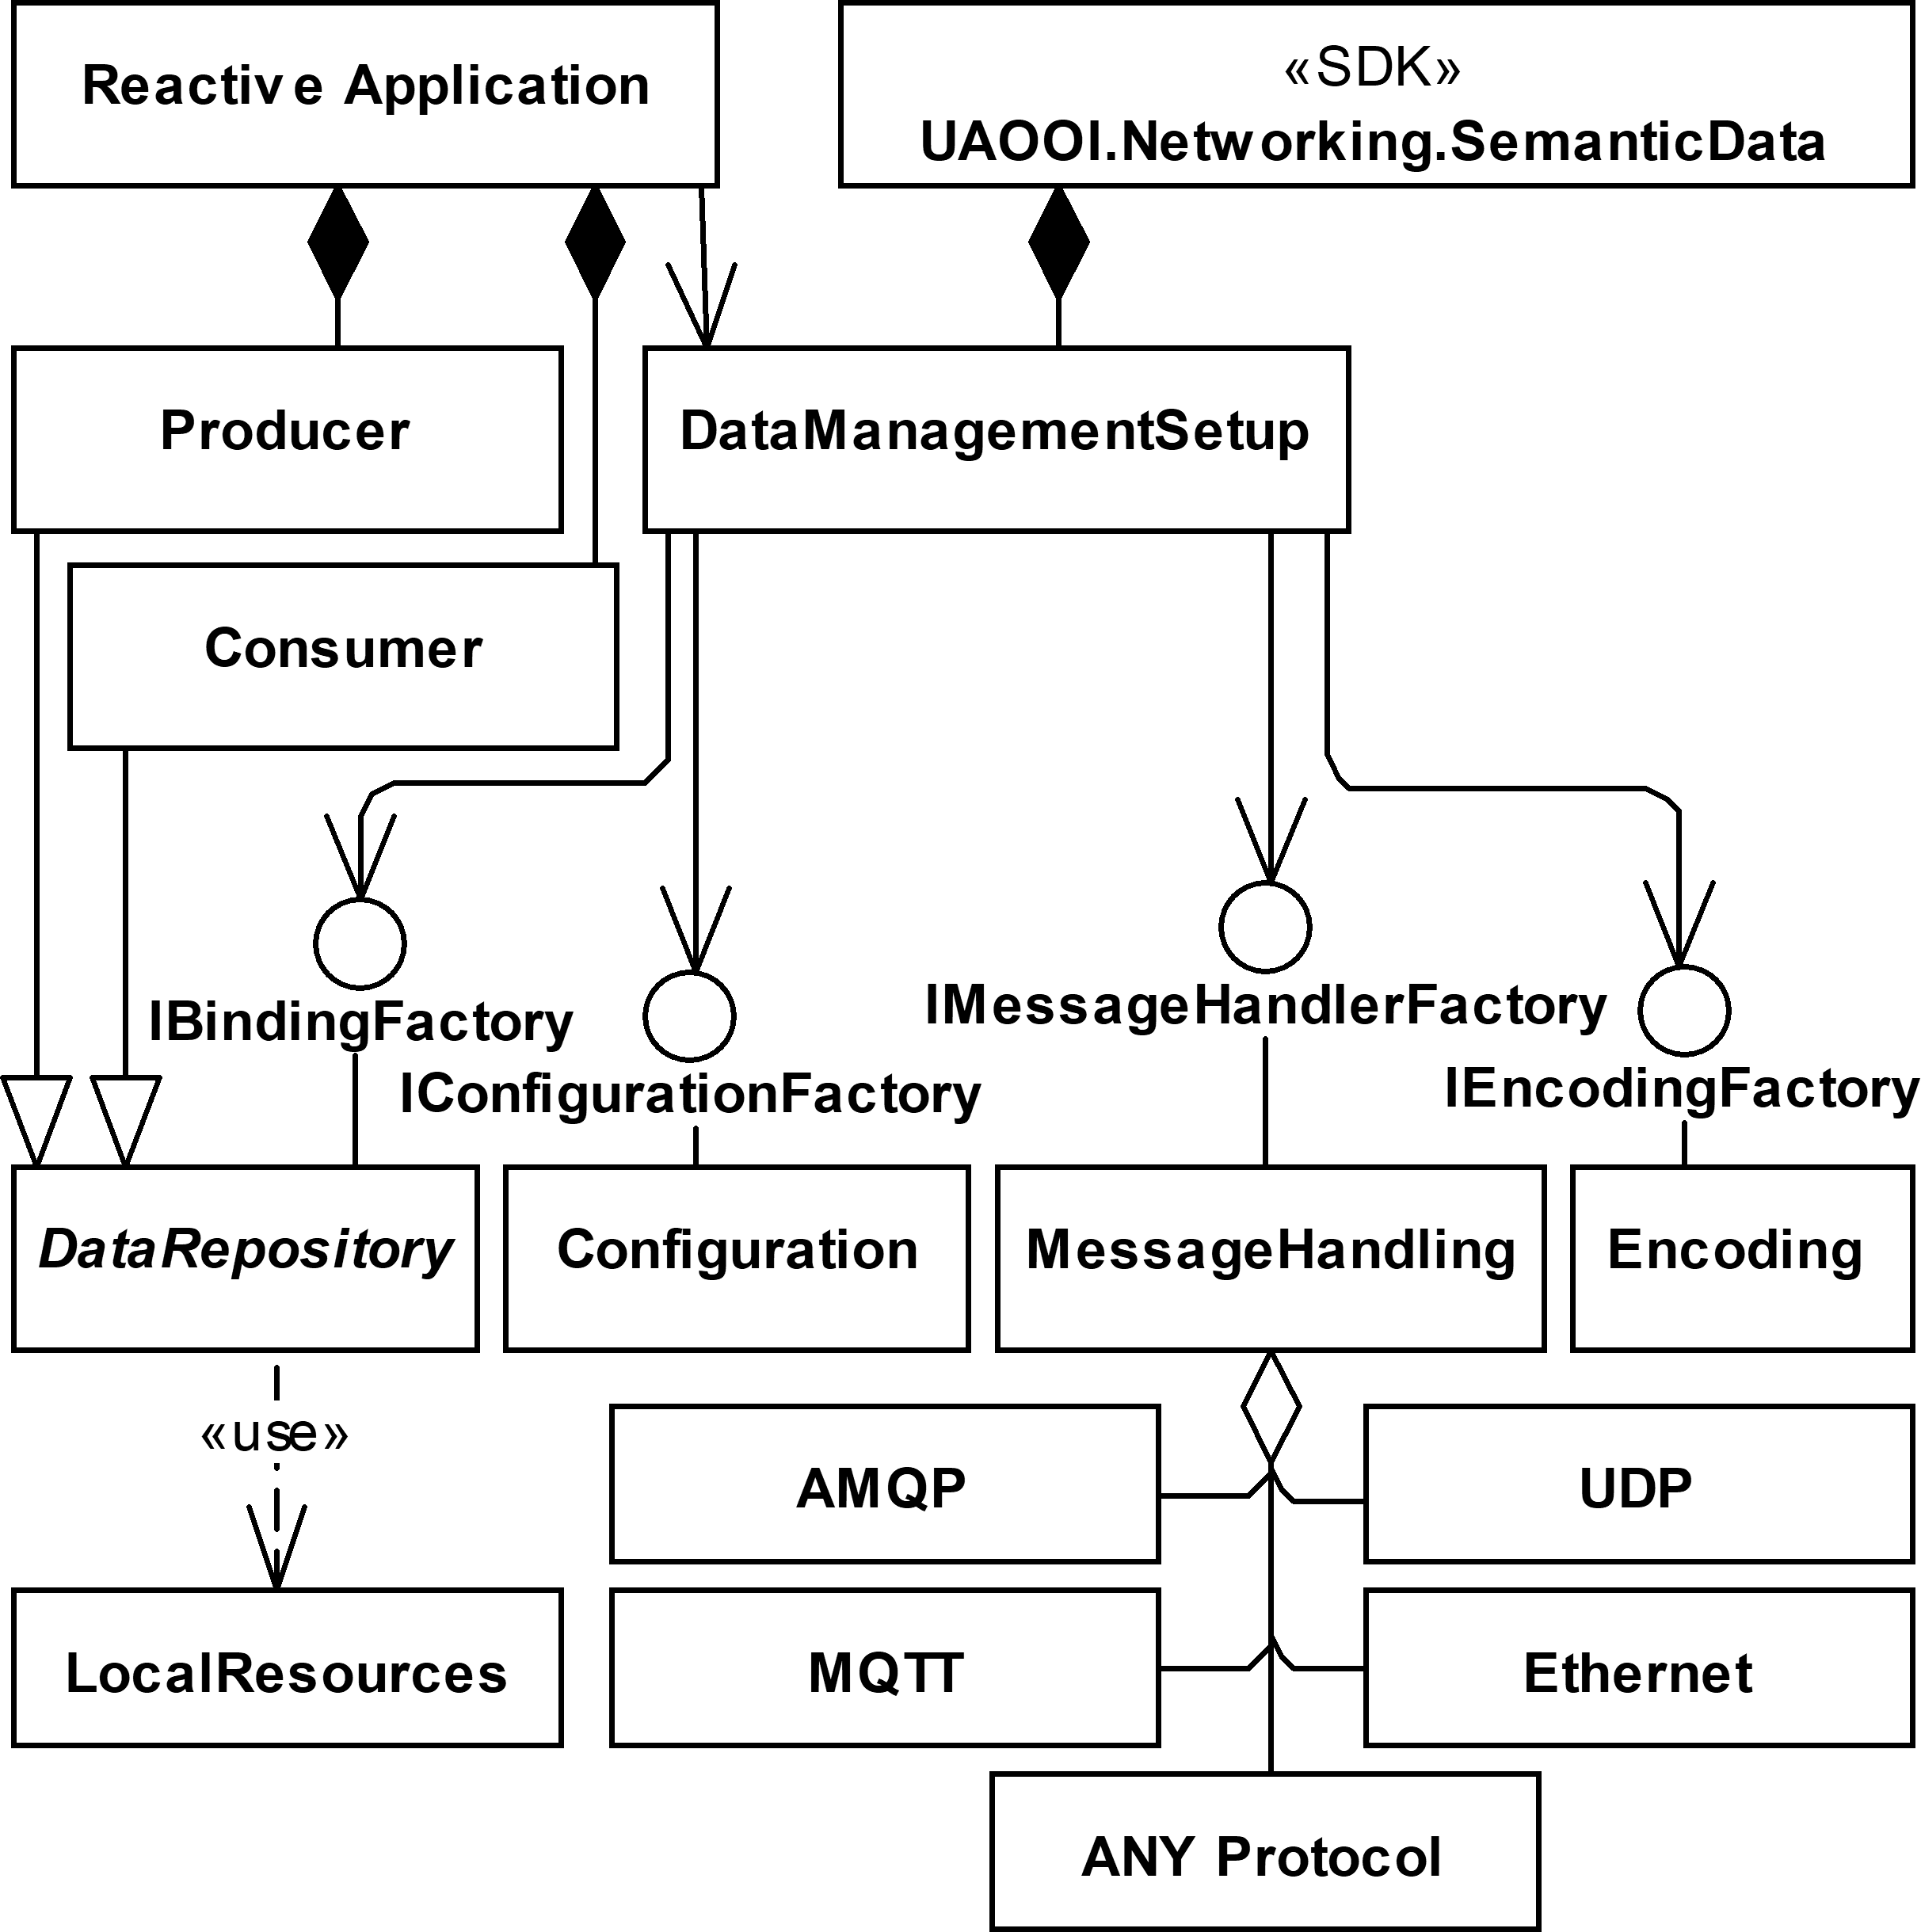
\includegraphics[width=0.53\textwidth]{UADataApplicationArchitecture.eps}
      \caption{Reactive interoperability architecture}\label{figure2.UADataApplicationArchitecture}
\end{wrapfigure}

From the above discussion, we can learn that the main design decisions must concern standardization and flexibility. Standardization needs the selection of an international interoperability specification to make the library ready to be adopted by the multi-vendor environment. Flexibility requires an architecture that promotes the polymorphic independent implementation of essential functions.

Piece by piece integration of a cyber-physical system using multi-vendor products requires that M2M communication employs international standards as the interoperability foundation. OPC Unified Architecture Part 14 PubSub has been selected in this respect (Sect. \ref{cloud-to-sensors-field-level-connectivity}). By design, this standard should support the required publisher-subscriber communication pattern. It must be stressed that the specification provides only an abstract interoperability definition. Abstract means that the standard must not limit the implementation strategy.

Many parts in the domain model presented in Fig.~\ref{figure2.UADataApplicationArchitecture} requires a polymorphic approach to implementation. To promote the polymorphic ready solution the following concepts have been adopted:

\begin{itemize}
      \item \textbf{separation of concerns} - to allow an independent development of the parts~\cite{RefWorks:doc:5d92609be4b02eb43d372bd1}
      \item \textbf{dependency injection} - to allow late binding of separately implemented parts~\cite{RefWorks:doc:5d925b77e4b030b4e0596f5d}
\end{itemize}

To promote the polymorphic approach, the library has a factory class called \emph{DataManagementSetup} that is a placeholder to gather all injection points used to compose external parts. To be injected the parts must be compliant with an appropriate contract expressed as the following interfaces:

\begin{itemize}
      \item \emph{IBindingFactory} - bidirectional data exchange with the underlying process
      \item \emph{IConfigurationDataFactory} - the configuration data access
      \item \emph{IMessageHandlerFactory} - \textbf{Message} entities pushing to/pulling from the wire
      \item \emph{IEncodingFactory} - searching a dictionary containing value converters
\end{itemize}

It is expected that the functionality implementation expressed by these interfaces is provided as independent external composable parts. The composition is accomplished at run time, and the effective application functionality depends essentially on reusable loosely coupled parts composed applying the dependency injection software engineering and adaptive programming concept \cite{RefWorks:doc:5d9796cbe4b0f66c52dccf04}.

The \emph{DataRepository} represents data holding assets in the \emph{Reactive Application} implementing the \emph{IBindingFactory} interface. It captures functionality responsible for accessing the external process data from \emph{LocalResources}. The \emph{LocalResources} represents an external part that has a very broad usage purpose. For example, it may be any kind of the process data source/destination, i.e. raw data (e.g. PLC internal registers), OPC UA Address Space Management \cite{mpostol2020}, cloud, file, database, graphical user interface, to name only a few.

Depending on the expected network role the library supports the implementation of:

\begin{itemize}
      \item \emph{Consumer} - entities processing data from incoming messages,
      \item \emph{Producer} - entities gathering process data and populating outgoing messages.
\end{itemize}

The \emph{Consumer} and \emph{Producer} classes are derived from the \emph{DataRepository} (Fig.~\ref{figure2.UADataApplicationArchitecture}). The \emph{Consumer} uses the \emph{IBindingFactory} to gather the data recovered from the \emph{Message} instances pulled from a network. The received data may be processed or driven to any data destination, e.g. cloud-based front-end. The \emph{Producer} mirrors the \emph{Consumer} functionality and, after reading data from an associated source, populates the \emph{Message} using the gathered data.

By design, the \emph{DataRepository} and associated entities, i.e.~\emph{Local Resources}, \emph{Consumer}, \emph{Producer} are embedded in external parts, and consequently, the application scope may cover practically any concern that can be separated from the core \emph{Reactive Application} implementation.

The application startup phase concerns all the parts composed to make a running instance of the application program using the dependency injection approach to allow separate development and late binding. This approach makes any modification straightforward at any development and maintenance stage. From the end-user point of view, the composition process of the running program using independently developed parts is invisible. Because in any case a single program instance is created in a typical approach, we shall expect a commonly shared configuration mechanism providing mutually exclusive parameters to separately developed parts. This scenario has been addressed by the proposed implementation thanks to making the configuration expandable.

\begin{wrapfigure}{t}{0.55\textwidth}
      \centering
      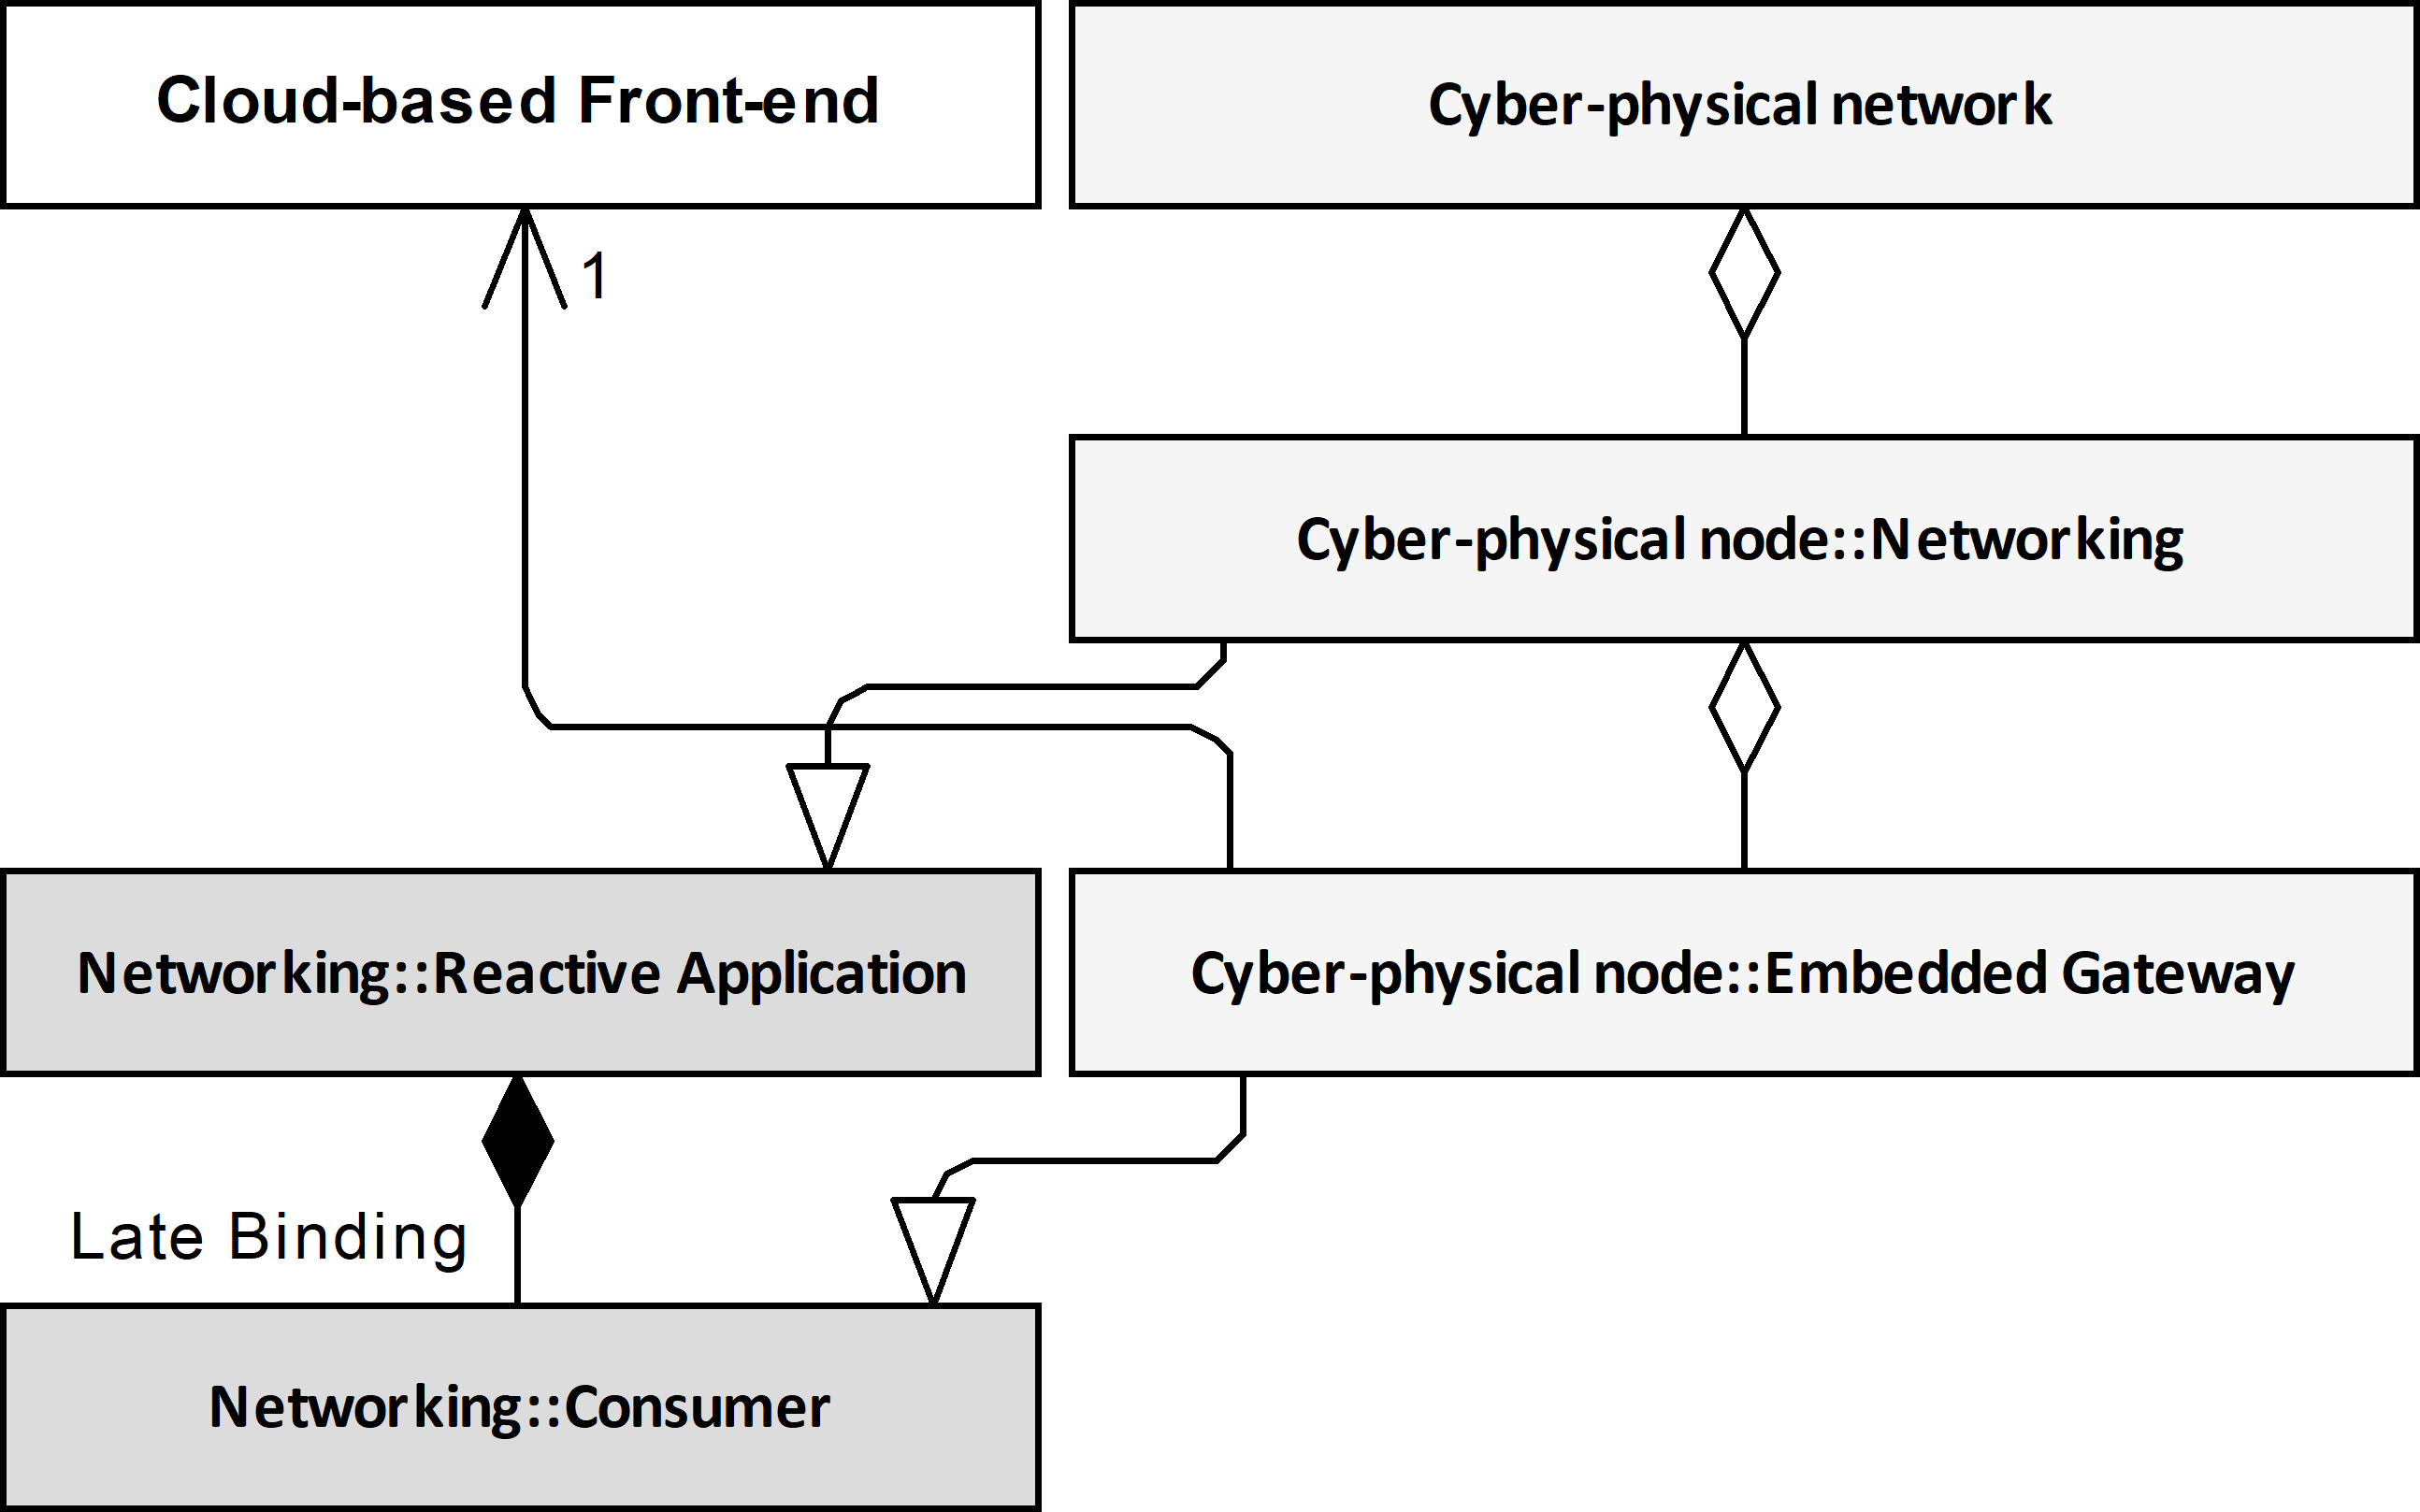
\includegraphics[width=0.53\textwidth]{ImplementationDomainModel.eps}
      \caption{Architecture Domain Model}\label{figure3.ImplementationDomainModel}
\end{wrapfigure}

From the discussion covered by the Sect. \ref{cloud-to-sensors-field-level-connectivity} we can infer that the interoperability of communicating parties requires establishing a semantic-context and security-context between them. If the received data is driven to any external data destination (e.g. cloud-based front-end) using out-of-band protocol semantic-context and security-context must be defined for this interoperability relationship. There are a vast variety of possibilities for how to define these contexts. Anyway, the most common starting point is the configuration. The proposed approach to instantiate the application as a set of composable parts is very useful in this respect because it makes it possible to expand the core configuration functionality and adapt it to be helpful also in this case. Therefore, the semantic-context may be created based on the configuration using the implementation of the \emph{IConfigurationDataFactory} interface.

Concluding, decoupling of this functionality implementation using an abstract contract and late binding mechanism allows:

\begin{itemize}
      \item implementation of practically any configuration management scenario,
      \item modification of this functionality later after releasing the library or deploying the application program in the production environment.
\end{itemize}

\section{Azure - OOI Interoperability Implementation}\label{section.gateway-implementation}


A generic domain model presenting interconnection architecture between the Azure \emph{Cloud-based\ Front-end} and \emph{Cyber-physical\ node} attached to the \emph{Cyber-physical\ network} is presented in Fig.~\ref{figure1.StrategyDomainModel}. It is proposed to implement the \emph{Cyber-physical\ node} by adopting the \emph{Reactive Application} archetype compliant with the reactive interoperability concept (Fig. \ref{figure2.UADataApplicationArchitecture}) described in the Sect. \ref{ooi-main-technology-features}. Merging selected entities of this archetype into the proposed domain model (Fig. \ref{figure1.StrategyDomainModel}) lead to a model expressed as the diagram presented in Fig. \ref{figure3.ImplementationDomainModel}. In the proposed approach the \emph{Embedded Gateway} is derived from the \emph{Consumer} role implemented as as a composable part aggregated by the \emph{Reactive Application}.

\hyphenation{PartData-Mana-gement-Setup}

In the final deployment architecture (Fig. \ref{figure4.ImplementationArchitecture}) the \emph{Consumer} role has been realized by the \emph{PartDataManagementSetup} that is derived from \emph{DataManagementSetup} provided by the library. \emph{Networking} (SDK) was removed from this diagram for the sake of simplicity. Instantiating \emph{PartDataManagementSetup} is the first step for bootstrapping process of the \emph{Consumer} role functionality. This class provides an entry point to initialize all properties, which are injection points of all parts composing this role. It extends the functionality of the \emph{DataManagementSetup} based on the following associated classes:

\begin{itemize}
      \item \emph{PartConfigurationFactory} - to get access to the application configuration
      \item \emph{PartBindingFactory} - to gather the data recovered from the \emph{Message} instances pulled from the wire
      \item \emph{CommunicationContext} - to handle communication with the Azure services
\end{itemize}

In this case, the implementation of the \emph{IConfigurationFactory} interface is based entirely on the \emph{Networking} library. The implementation provided by the library is generic, but it is flexible enough to meet all the requirements, which warrants no need for further modifications for adoption. It is ready to provide all necessary configuration parameters to establish semantic and security contexts related to Azure interoperability.

\begin{figure}
      \centering
      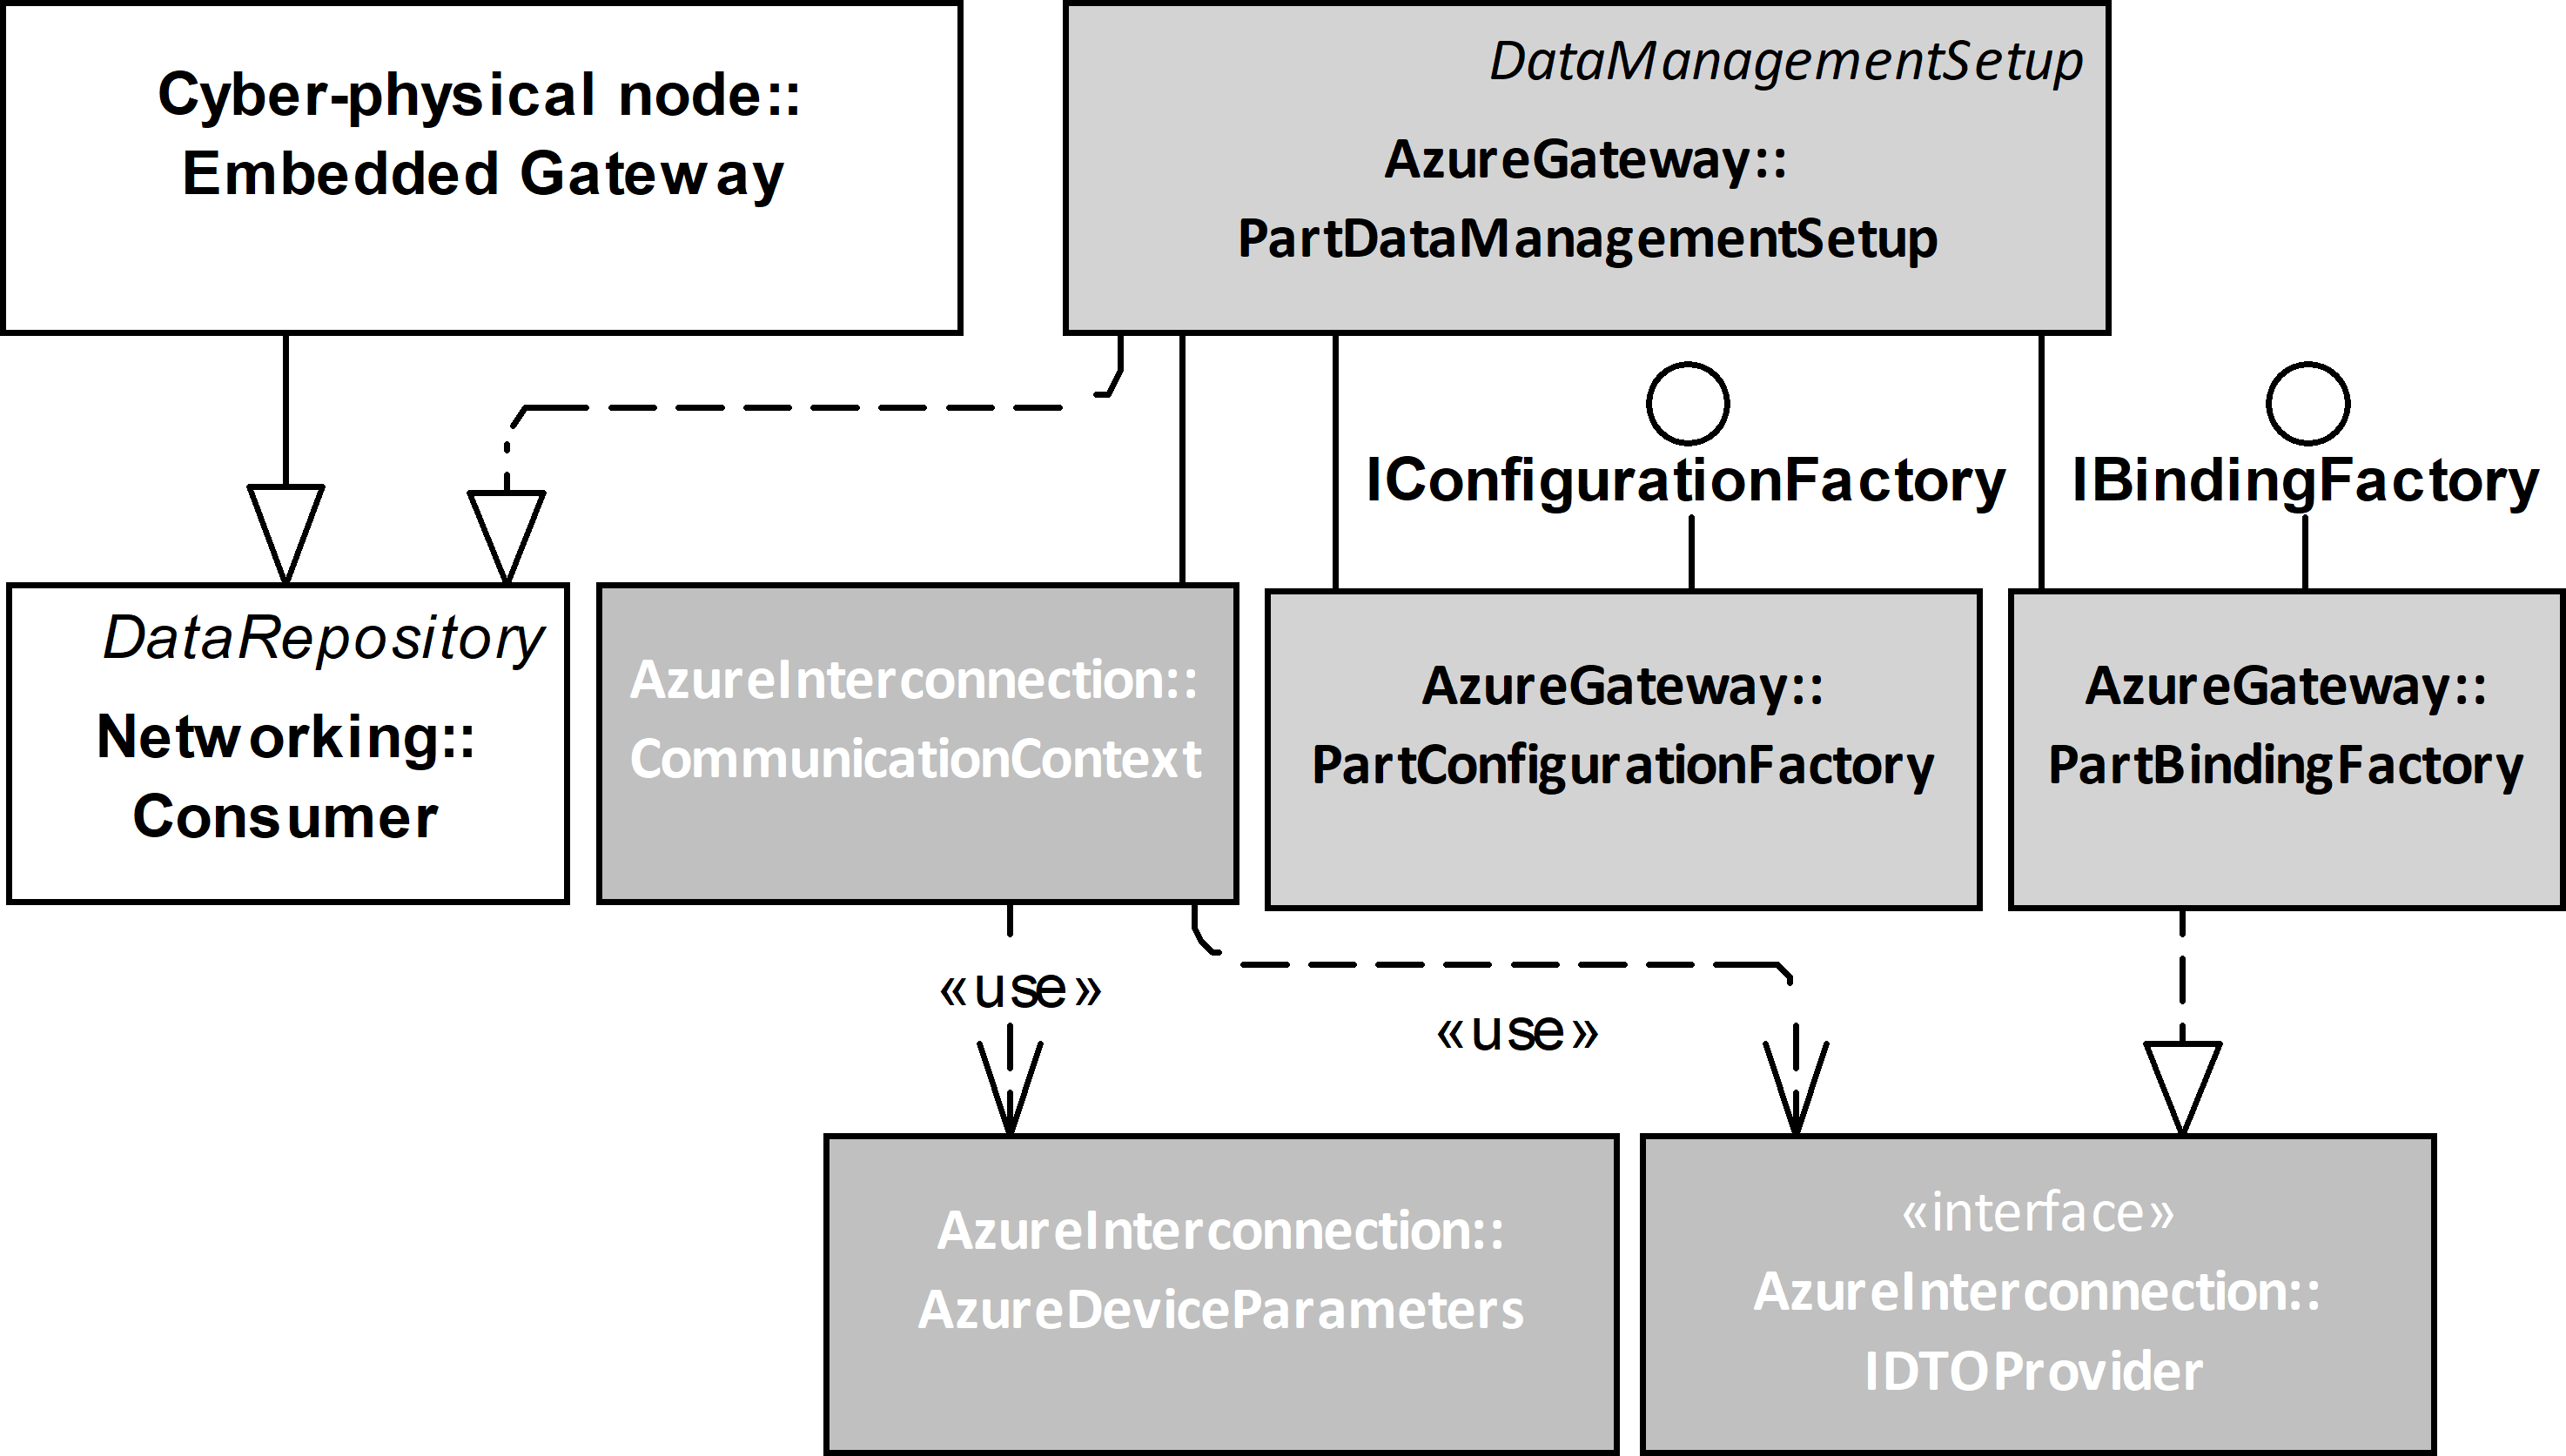
\includegraphics[width=11cm]{ImplementationArchitecture.eps}
      \caption{Implementation Architecture}\label{figure4.ImplementationArchitecture}
\end{figure}

The \emph{PartBindingFactory} implements the \emph{IBindingFactory} to gather the data recovered from the \emph{Message} instances pulled from a network. The received data is driven to \emph{CommunicationContext} for further encoding and finally pushing it to the Azure services using the configured out-of-band protocol.

\emph{IEncodingFactory} and \emph{IMessageHandlerFactory} interfaces (Fig. \ref{figure2.UADataApplicationArchitecture}) have been implemented in independent libraries and ae not considered for any modifications to deploy \emph{Embedded Gateway} functionality. The current implementation of the mentioned interfaces is localized at run time as services using an instance of the \emph{IServiceLocator}\footnote{ \url{https://www.nuget.org/packages/CommonServiceLocator} }. In this example, it is assumed that \emph{IServiceLocator} is implemented to resolve references to any external services. Both interfaces are used to manage the interconnection of the node with the \emph{Cyber-physical Network}.

The Azure interconnection is realized using the \emph{CommunicationContext}. It implements a message encoder and establishes the out-of-band communication stack.

The recovered data from the \emph{Message} is obtained from the \emph{PartBindingFactory} using the \emph{IDTOProvider} that defines a contract used to pull the Data Transfer Object created from a subscription by the \emph{PartBindingFactory}. The transfer process requires data conversion from source to destination encoding, i.e. replacing bitstreams used by the CPS with equivalent ones for the cloud-based services. The Azure offers a vast variety of built-in types ready to be used in common cases, but not necessarily there are equivalent counterparts in use by the CPS. The Azure uses JSON based Data Transfer Object encoding and schema defined based on the solution metadata. The PubSub uses JSON and binary Data Transfer Object encodings. In any case, the data recovered from the Message pulled from a subscription is stored locally using the object model based on standard .NET types. \emph{PartBindingFactory} maps selected object graph onto the JSON message required by the cloud services.

%TBD
The Azure supports HTTP, AMQP, and MQTT protocol stacks, which are all standard ones. Consequently, it is possible to apply any available implementation compliant with an appropriate specification to achieve connectivity. In this case, all parameters required to establish semantic and security contexts are up to the gateway responsibility. Alternatively, the API offered by the dedicated frameworks (libraries) may be used. Using a framework the configuration process may be reduced significantly, and the communication protocol selection has only an indirect impact on the interoperability features. The Azure interconnection may be obtained using the following \emph{Microsoft.Azure} packages:

\begin{itemize}
      \item \emph{Devices} - Service SDK for Azure IoT Devices
      \item \emph{Devices.Client} - Device SDK for Azure \emph{IoT\ Hub} including dependencies implementing MQTT and AMQP communication
      \item \emph{Devices.Shared} - Common code for Azure IoT Device and Service SDK
      \item \emph{Devices.Provisioning.Client} - Provisioning Device Client SDK for Azure IoT Devices
      \item \emph{Devices.Provisioning.Transport.*} - Provisioning Device Client Transports (HTTPS, AMQP, MQTT) for Azure IoT Devices
\end{itemize}

%____________________

The encoded JSON messages must be transferred over the network to Azure using the selected protocol stack. The Azure supports standard protocols. Consequently, it is possible to apply any available implementation compliant with an appropriate specification to achieve connectivity. In the proposed gateway implementation, the Azure interconnection has been obtained using the packages described in Sect.

Azure and PubSub use different security mechanisms so in the proposed solution establishing security-context is realized independently. The \emph{CommunicationContext} is responsible to establish this context as an embedded negotiation phase tightly coupled with establishing interconnection.

\section{Conclusion}\label{section.conclusion}

Nowadays, the macro optimization of the industrial processes requires an integration of a vast variety of distributed applications provided by Information and Communication Technology. It requires further research on the integration of \textbf{machine - centric} Cyber-Physical Systems (CPS) with \textbf{human - centric} front-end in the context of new emerging disciplines, i.e. Industry 4.0 and the Industrial Internet of Things (Sect. \ref{introduction}).

CPS is composed using the multi-vendor components (data holding assets) interconnected atop of the Machine To Machine (M2M) communication. In many applications, the dynamic nature of the CPS must be considered. Dynamic nature means that interconnected assets may be added/removed from the network at any time. By design, typically CPS must fulfill the real-time and mobility of the assets requirements.

Highly-distributed solutions used to control/monitor a set of geographically dispersed islands of automation (e.g. virtual power plants producing renewable energy) additionally must leverage public communication infrastructure, namely the Internet. If islands of automation must be controlled over the Internet, the cloud computing concept may be recognized as a reasonable answer. Following this concept, the cloud-based supervisory control functionality is applied as a set of services employing abstraction and virtualization - two main pillars of the cloud computing paradigm. In the cloud computing concept, virtualization is recognized as the possibility to share the services by many users, and abstraction hides implementation details.

The main goal of this research is working out a new generic architecture and deployment scenario applicable for the integration of the \textbf{machine-centric} CPS and emerging cloud computing as a \textbf{human-centric} front-end.

If we must bother with the network traffic propagation asymmetry or mobility of the asset network attachment-points the reactive relationship \cite{mpostol2020} could alleviate the challenges posed by the interactive approach. The real-time multi-vendor environment makes communication standardization especially important. To support this environment, OPC Unified Architecture \cite{RefWorks:doc:5ac86c98e4b009947bbb874c} interoperability standard has been selected. As it was pointed out in the Sect. \ref{cloud-to-sensors-field-level-connectivity} using OPC UA PubSub \cite{RefWorks:doc:5d98837de4b055984c0eecf0} the aggregation of nodes by the network is loosely coupled, i.e. nodes can be added and removed from the network dynamically, and nodes may represent mobile data holding assets.

From the analysis covered by the Sect. \ref{cloud-to-sensors-field-level-connectivity} it is concluded that the \emph{Embedded Gateway} archetype best suits all requirements described above. It relaxes most of the issues related to \textbf{direct interconnection} and solutions inferred from the middleware concept, i.e. \textbf{edge device} - remote cloud agent and \textbf{field level gateway} - a dedicated custom agent. Additionally, it could be used to connect to many independent clouds at the same time. The generic domain model for the proposed interconnection archetype is presented in the Fig.~\ref{figure1.StrategyDomainModel}. We have highlighted that to promote the separation of concern design principle, the gateway functionality should be implemented as a self-contained dedicated software part embedded in the core \emph{Networking} service of the \emph{Cyber-physical\ node}. The main functionality of this component is to transfer process data between \emph{Cyber-physical\ network} using \emph{Networking} services of an existing \emph{Cyber-physical\ node} and \emph{Cloud-based\ front-end} using officially supported by the cloud vendor interconnection services.

To promote interoperability and address the demands of the M2M communication in the context of a multi-vendor environment the prototyping should use a framework that must be compliant with the OPC UA Part 14 PubSub (Sect. \ref{cloud-to-sensors-field-level-connectivity}) and support the \emph{Reactive Interoperability} (Sect. \ref{introduction}) concept. We proposed to use an open-source library named \emph{UAOOI.Networking} (\emph{Networking} for short) (Fig.~\ref{figure2.UADataApplicationArchitecture}) for this purpose. It is worth stressing that based on this approach only dedicated functionality related to the communication with the cloud must be implemented.

We derived the final model presented in Fig. \ref{figure4.ImplementationArchitecture} by merging selected entities from the \emph{Networking} library (Fig.~\ref{figure2.UADataApplicationArchitecture}) into the generic interconnection domain model (Fig. \ref{figure1.StrategyDomainModel}). In the proposed approach the \emph{Embedded Gateway} is derived from the \emph{Consumer} role implemented as as a composable part aggregated by the \emph{Reactive Application}.

The proposals are backed by proof of concept reference implementations. Prototyping addresses Microsoft Azure cloud as an example. The outcome has been just published on GitHub as the open-source (MIT licensed) repository. The proposed solutions have been harmonized with the more general concept called the Object-Oriented Internet.

The described results prove that the \emph{Embedded Gateway} archetype implementation is possible based on the existing standalone framework supporting reactive interoperability atop the M2M communication compliant with the OPC UA PubSub standard. It is worth stressing that there is no dependency on the Client/Server session-oriented relationship. This relationship is in contrast to the architecture described in the OPC UA Part 1 \cite{OPCUAPart1} specification where the publisher role is tightly coupled with the \textbf{Address Space} \cite{RefWorks:doc:5ac86c97e4b009947bbb8728} embedded component of the OPC UA Server. The real challenge of the future work is to prove that the proposed solution is flexible enough to be used as an archetype to inject the \emph{Embedded Gateway} part into the OPC UA Client/Server to get connected with the cloud in case of the interactive relationship.

In the proposed approach the cloud interoperability is obtained by implementing a dedicated part employing out-of-band communication only without dependency on the OPC UA functionality at all. It is worth stressing that the gateway functionality is implemented as a part - composable to the whole without programming skills. Because the part is composed at the runtime it makes it possible to modify its functionality later after releasing the library or even deploying the application program in the production environment.

Concluding, the paper describes a proof of the concept that applying the proposed architecture and deployment scenario it is possible to integrate cloud services (e.g. \textbf{Azure\ IoT\ Central}) with the \emph{Cyber-physical network} interconnected as one whole atop of the OPC UA PubSub. It is in contrast to interconnecting cloud-based front-end services with the \emph{ Address\ Space} instance exposed by a selected OPC UA server limiting the PubSub role to data exporter transferring the data out of the OPC UA ecosystem.

\bibliography{ICCS21MPostoOOIGateway2Azure}
\bibliographystyle{splncs04}

\end{document}
